
\documentclass[11pt]{article}


% Use wide margins, but not quite so wide as fullpage.sty
\marginparwidth 0.2in 
\oddsidemargin 0.1in 
\evensidemargin 0.1in 
\marginparsep 0.1in
\topmargin 0.1in 
\textwidth 6.5in \textheight 8 in
% That's about enough definitions

% multirow allows you to combine rows in columns
\usepackage{multirow}
% tabularx allows manual tweaking of column width
\usepackage{tabularx}
% longtable does better format for tables that span pages
\usepackage{longtable}
\usepackage{booktabs}
\usepackage{graphicx}
\usepackage{amssymb} % needed for math
\usepackage{amsmath} % needed for math
\usepackage{listings} % needed for the inclusion of source code
%\usepackage{mips}
\usepackage{color}
% this is needed for forms and links within the text
\usepackage{hyperref}  
\usepackage{xcolor}
\usepackage{listings}
\definecolor{vgreen}{RGB}{104,180,104}
\definecolor{vblue}{RGB}{49,49,255}
\definecolor{vorange}{RGB}{255,143,102}
\usepackage{courier} %% Sets font for listing as Courier.
\lstset{
tabsize = 4, %% set tab space width
showstringspaces = false, %% prevent space marking in strings, string is defined as the text that is generally printed directly to the console
numbers = left, %% display line numbers on the left
commentstyle = \color{green}, %% set comment color
keywordstyle = \color{blue}, %% set keyword color
stringstyle = \color{red}, %% set string color
rulecolor = \color{black}, %% set frame color to avoid being affected by text color
basicstyle = \small \ttfamily , %% set listing font and size
breaklines = true, %% enable line breaking
numberstyle = \tiny,
}


\makeatletter
\newcommand*\@lbracket{[}
\newcommand*\@rbracket{]}
\newcommand*\@colon{:}
\newcommand*\colorIndex{%
    \edef\@temp{\the\lst@token}%
    \ifx\@temp\@lbracket \color{black}%
    \else\ifx\@temp\@rbracket \color{black}%
    \else\ifx\@temp\@colon \color{black}%
    \else \color{vorange}%
    \fi\fi\fi
}
\makeatother

\usepackage{trace}

\begin{document}
% this is an alternate method of creating a title
%\hfill\vbox{\hbox{Gius, Mark}
%       \hbox{Cpe 456, Section 01}  
%       \hbox{Lab 1}    
%       \hbox{\today}}\par
%
%\bigskip
%\centerline{\Large\bf Lab 1: Security Audit}\par
%\bigskip
%\author{Name Surname, Student ID}
%\title{BBM233: Logic Design Lab\\2020 Fall\\Lab Experiment \#(add experiment no. here) Report}
%\maketitle


\begin{titlepage}
\newcommand{\HRule}{\rule{\linewidth}{0.5mm}}

\center


\includegraphics[width=0.2\textwidth]{logo.png}
\vfill
\textsc{\LARGE Hacettepe University}\\[0.5cm]
\textsc{\Large Computer Engineering Department}\\[1.5cm]
\textsc{\large BBM204 Software Practicum II - 2024 Spring}\\[0.5cm]

\HRule \\[0.4cm]
{ \huge \bfseries Programming Assignment 1}\\[0.4cm] 
\HRule \\[0.3cm]
{\large \today}\\[2cm]
\begin{minipage}{0.4\textwidth}
\begin{flushleft} \large
\emph{Student name:}\\
Name \textsc{Surname}
\end{flushleft}
\end{minipage}
\begin{minipage}{0.4\textwidth}
\begin{flushright} \large
\emph{Student Number:} \\
b00000000
\end{flushright}
\end{minipage}\\[2cm]
\vfill
\end{titlepage}



\section{Problem Definition}

Briefly state the problem that you are trying to solve. Add any background information if necessary.


\section{Solution Implementation}

Your answers, explanations, code go into this section.

\subsection{Sorting Algorithm 1}

Example how to add Java code:

\begin{lstlisting}[language = Java , frame = trBL , firstnumber = last , escapeinside={(*@}{@*)}]
public class Factorial {
    public static void main(String[] args) {
        final int NUM_FACTS = 100;
        for(int i = 0; i < NUM_FACTS; i++)
            System.out.println( i + "! is " + factorial(i));
    }
    public static int factorial(int n) {   
        int result = 1;
        for(int i = 2; i <= n; i++) (*@\label{for}@*)
            result *= i;
        return result;
    }
}
\end{lstlisting}

And you can reference line \ref{for} in the code like this.

\subsection{Sorting Algorithm 2}

Example how to add Java code:

\begin{lstlisting}[language = Java , frame = trBL , firstnumber = last , escapeinside={(*@}{@*)}]
public class Factorial {
    public static void main(String[] args) {
        final int NUM_FACTS = 100;
        for(int i = 0; i < NUM_FACTS; i++)
            System.out.println( i + "! is " + factorial(i));
    }
    public static int factorial(int n) {   
        int result = 1;
        for(int i = 2; i <= n; i++) (*@\label{for}@*)
            result *= i;
        return result;
    }
}
\end{lstlisting}

And you can reference line \ref{for} in the code like this.

\section{Results, Analysis, Discussion}

Your explanations, results, plots go in this section...

Running time test results for sorting algorithms are given in Table \ref{tab:results}. 

\begin{table}[ht!]
\centering
\caption{Results of the running time tests performed for varying input sizes (in ms).}
\label{tab:results}
\resizebox{\textwidth}{!}{%
\scriptsize
\begin{tabular}{|l|l|l|l|l|l|l|l|l|l|l|} \hline
\multicolumn{1}{c}{\multirow{2}{*}{\textbf{}}} & \multicolumn{10}{c}{\textbf{Input Size $n$}}                                       \\ \hline
\multicolumn{1}{|c|}{\textbf{Algorithm}}                           & \textbf{500} & \textbf{1000} & \textbf{2000} & \textbf{4000} & \textbf{8000} & \textbf{16000} & \textbf{32000} & \textbf{64000} & \textbf{128000} & \textbf{250000} \\  \hline
                                               & \multicolumn{10}{c|}{\textbf{Random Input Data Timing Results in ms}}                                    \\ \hline
Insertion sort                                 &     &      &      &      &      &       &       &       &        &        \\ \hline
Merge sort                                     &     &      &      &      &      &       &       &       &        &        \\ \hline
Counting sort                                    &     &      &      &      &      &       &       &       &        &        \\ \hline
                                               & \multicolumn{10}{c|}{\textbf{Sorted Input Data Timing Results in ms}}                                    \\ \hline
Insertion sort                                 &     &      &      &      &      &       &       &       &        &        \\ \hline
Merge sort                                     &     &      &      &      &      &       &       &       &        &        \\ \hline
Counting sort                                    &     &      &      &      &      &       &       &       &        &        \\ \hline
                                               & \multicolumn{10}{c|}{\textbf{Reversely Sorted Input Data Timing Results in ms}}                          \\ \hline
Insertion sort                                 &     &      &      &      &      &       &       &       &        &        \\ \hline
Merge sort                                     &     &      &      &      &      &       &       &       &        &        \\ \hline
Counting sort                                    &     &      &      &      &      &       &       &       &        &       \\ \hline
\end{tabular}
}
\end{table}


Running time test results for search algorithms are given in Table \ref{tab:searchresults}. 

\begin{table}[ht!]
\centering
\caption{Results of the running time tests of search algorithms of varying sizes (in ns).}
\label{tab:searchresults}
\resizebox{\textwidth}{!}{%
\scriptsize
\begin{tabular}{|l|l|l|l|l|l|l|l|l|l|l|} \hline
\multicolumn{1}{c}{\multirow{2}{*}{\textbf{}}} & \multicolumn{10}{c}{\textbf{Input Size $n$}}                                       \\ \hline
\multicolumn{1}{|c|}{\textbf{Algorithm}}                           & \textbf{500} & \textbf{1000} & \textbf{2000} & \textbf{4000} & \textbf{8000} & \textbf{16000} & \textbf{32000} & \textbf{64000} & \textbf{128000} & \textbf{250000} \\  \hline
                                             
Linear search (random data)                                  &     &      &      &      &      &       &       &       &        &        \\ \hline
Linear search (sorted data)                                      &     &      &      &      &      &       &       &       &        &        \\ \hline
Binary search (sorted data)                                    &     &      &      &      &      &       &       &       &        &        \\  \hline
\end{tabular}
}
\end{table}


Complexity analysis tables to complete (Table \ref{tab:resultscomplexity} and Table \ref{tab:spacecomplexity}):



    \begin{table}[!ht]
    \centering
    \caption{Computational complexity comparison of the given algorithms.}\label{tab:resultscomplexity}

    \begin{tabular}{llll}
    \toprule
    \textbf{Algorithm}       & \textbf{Best Case}       & \textbf{Average Case}    & \textbf{Worst Case}      \\ \toprule
    Insertion sort & $\Omega(n)$        & $\Theta(n^2)$       & $O(n^2)$       \\
    Merge sort     & $\Omega(n \log n)$ & $\Theta(n \log n )$ & $O(n \log n)$ \\
    Counting Sort     &         &      &      \\ 
    Linear Search     &         &      &      \\ 
    Binary Search     &       &         &    \\\bottomrule
    \end{tabular}
    \end{table}


    \begin{table}[!ht]
    \centering
    \caption{Auxiliary space complexity of the given algorithms.}\label{tab:spacecomplexity}

    \begin{tabular}{@{}ll@{}}
    \toprule
    \textbf{Algorithm}      & \begin{tabular}[c]{@{}l@{}}\textbf{Auxiliary Space}\\ \textbf{Complexity}\end{tabular} \\ \midrule
    Insertion sort & $O(1)$                     \\
    Merge sort     & $O(n)$                     \\
    Counting sort     &        \\ 
    Linear Search     &        \\ 
    Binary Search     &       \\\bottomrule
    \end{tabular}
    
    \end{table}



\newpage
Example how to include and reference a figure: Fig. \ref{fig:plot}.
    
    
    \begin{figure}[h!]
            \centering
            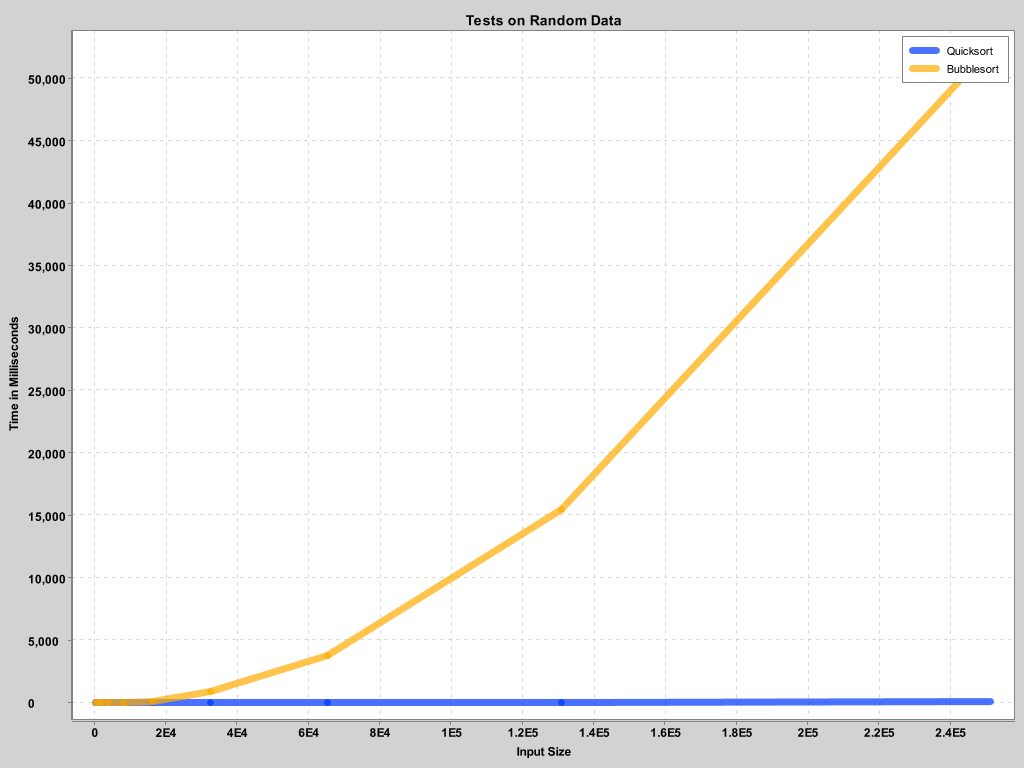
\includegraphics[width=\textwidth]{Tests on Random Data.png}
            \caption{Plot of the functions.}
            \label{fig:plot}
    \end{figure}


Example how to include and reference and resize figure: Fig. \ref{fig:plot2}.
    
    
    \begin{figure}[h!]
            \centering
            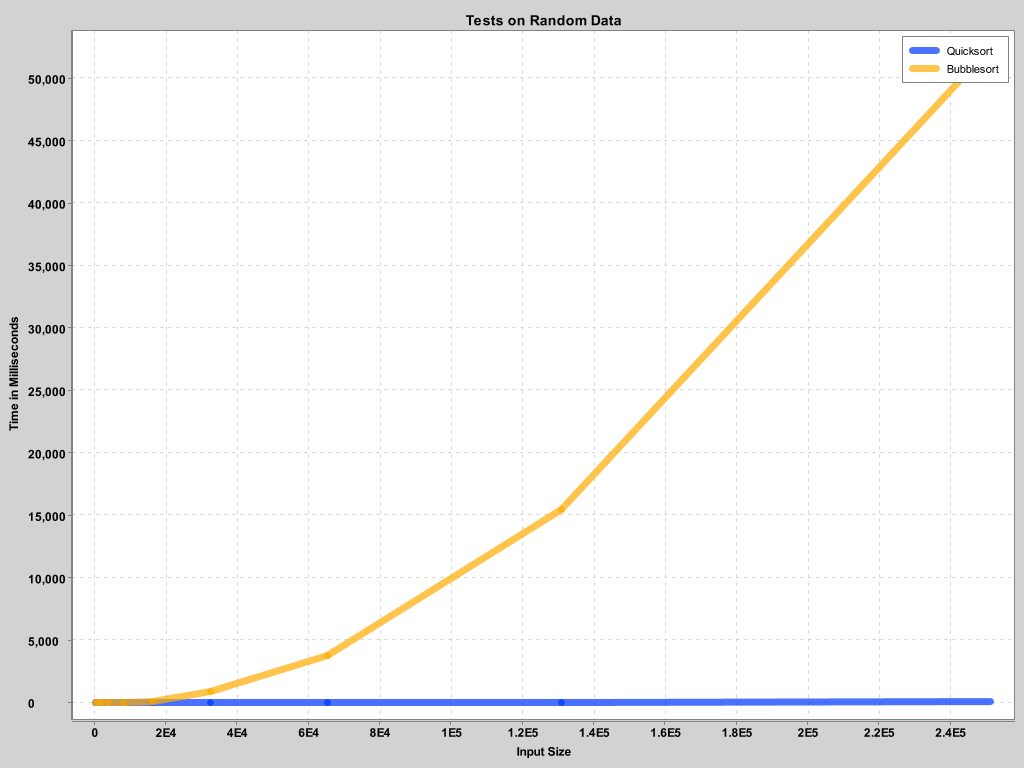
\includegraphics[width=0.7\textwidth]{Tests on Random Data.png}
            \caption{A smaller plot of the functions.}
            \label{fig:plot2}
    \end{figure}

    
Results analysis, explanations...



\section{Notes}

Here you can add your notes if any.



\section*{References}


\begin{itemize}
    \item {Reference 1...}
    \item {Reference 2...}
\end{itemize}


\end{document}
